\chapter{绘制垫片立体图}\label{chap:dianpian}
第二天晚上秦奋满脸微笑地来到父亲的书房。他父亲见他兴趣盎然,说道:看来你的收获不错,把你绘的立体图给我检验一下。

秦奋将白天画的立体一一打开给父亲看。他父亲看了后非常满意,于是又问道:你说说旋转建模法和拉伸建模法的区别。

秦奋:旋转建模法只适合回转体类零件的建模,而拉伸建模法不仅可以用于回转体类块零件的建模,也可以用于平面体类零件的建模。

爸爸:说得很对,你已经把两种方法的精髓都掌握了。

秦奋:我们今天学习什么零件的建模呢?

爸爸拿出一幅调压阀垫片零件图(图\ref{fig:tiaoyafadianpian}说道:我们今天学习垫片零件的三维建模。

\noindent
\begin{figure}[htbp]
\centering
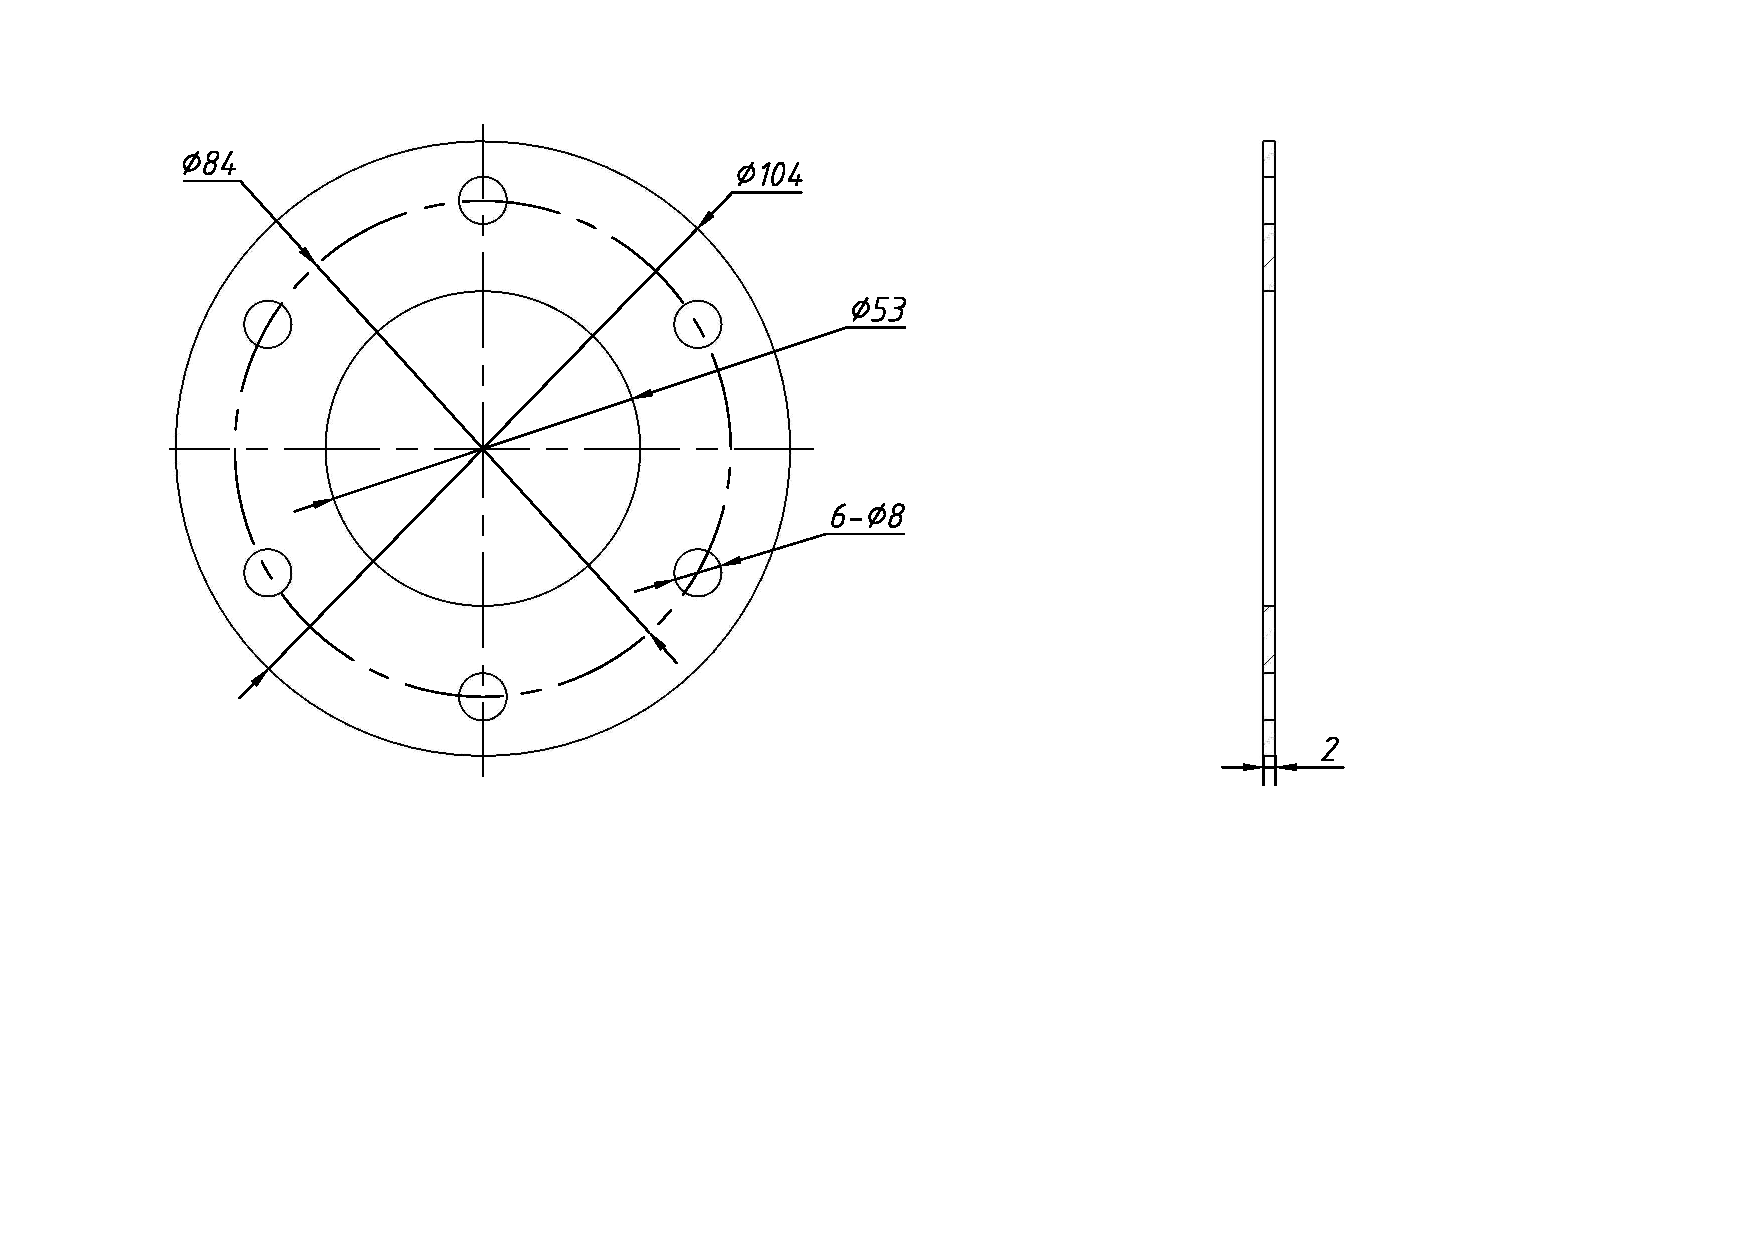
\includegraphics[scale=0.6]{tiaoyafadianpian.pdf}
\caption{垫片零件图}\label{fig:tiaoyafadianpian}
\end{figure}

秦奋看着零件图,皱眉道:昨天的零件图比较简单,图上所标注的尺寸关系我能够看懂,但今天的明显要困难一些。

爸爸:以后,我们将面对更加复杂的图形,其尺寸关系更加复杂,因此我们今天先了解平面图形分析方面的知识。
\endinput